\documentclass[tikz,convert, margin=3mm, 12pt]{standalone}
\usetikzlibrary{arrows}
\usepackage{pgfplots}
\pgfplotsset{compat=newest}


\begin{document}
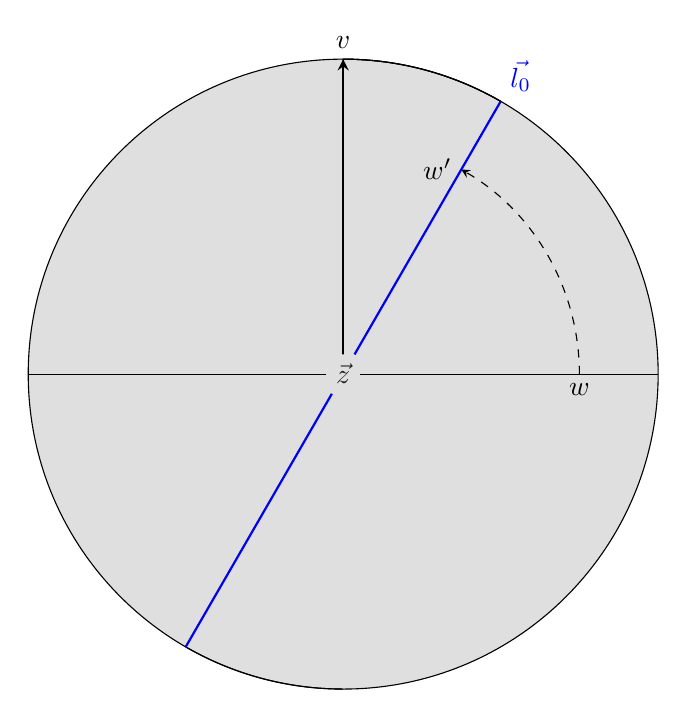
\begin{tikzpicture}

\node at (0,0) (z) {$\vec{z}$};


\draw[fill=gray, fill opacity=0.25, radius=4] (z) circle;
\draw[thick, -stealth] (z) -- (0,4) node[above] {$v$};
\draw (0,-4) arc[start angle = -90, delta angle= -30, radius=4] edge[blue, thick] (z);
\draw (z) -- (0,4) arc[start angle = 90, delta angle= -30, radius=4]  edge[blue, thick] (z);
\draw (z) -- (0,4) arc[start angle =90, delta angle=-30, radius=4]  node[blue, above right] {$\vec{l_0}$};

\draw (4,0) -- (z) -- (-4,0);
\draw[dashed, -stealth] (3,0) node[below] {$w$} arc[start angle = 0, delta angle = 60, radius =3] node[left] {$w'$};
\end{tikzpicture}
\end{document}
